\section{Quality evaluation}

The main errors in the final pipeline are introduced in the \match* step, and then reflected onto the \linkDDD*.
The main problem of the \match*  is the bubble density in the frames: with few bubbles, the epiline will not provide many candidates, thus making it easier to choose the correct match.
As the density increases, more candidates implies more chance for mistakes, which would become ``random, isolated bubbles'' in the 3D view, which also break the trajectories reconstructed by the \link*.

For measuring the quality as a function of the number of bubbles, different input datasets were developed in Blender, with the same format as the real data.
In these datasets, a number $N$ of bubbles rotate in circles around the center of the image, never exiting the field of view of any camera for the full 30 frame duration.
As such, the algorithm should be ideally able to reconstruct exactly $N$ tracklets with 30 frames of length.

A single matching error at frame $f$ will move one bubble into the wrong position, splitting the 30-frame trajectory into three, with lenghts $f$, $1$ and $29-f$.
As such, errors can be identified by examining the distribution of trajectory lenght.

Figure~\ref{fig:traj-len-distr} compares such distribution of lengths for $N$ values of 50, 100, 250, 1000.
The x axis represents the trajectory lenght, while the y axis is the percentage of bubbles associated with such lenght.
For example, a 30-frames trajectory would count as ``30 units'' in the x=30 bin, while a trajectory split at frame 5 would count as 5 units at x=5, 1 unit at x=1 and 24 units at x=24.
The percentage is obtained by dividing the value (in ``units'') of each bin by the total value of the graph, which is the total number of detected bubbles.
Iteally, the graph should have value 0\% for all bins other than 30, which should have a value of 100\%.
As visible in the graph, a good part of the trajectories is correct up to 100 bubbles, while adding more deteriorates the performance considerably.
The quality is therefore considered good up to 100 bubbles.

\begin{figure}
	\centerline{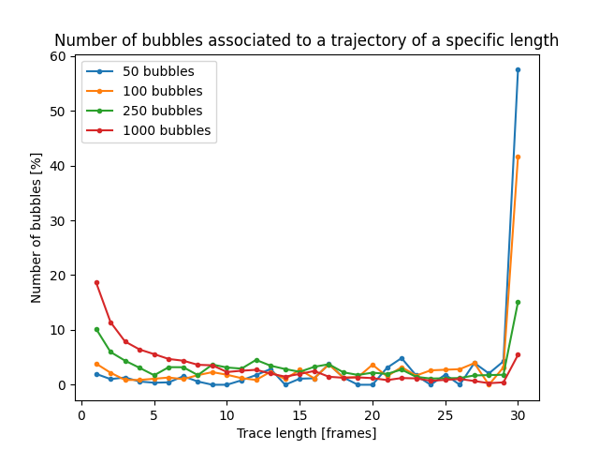
\includegraphics[width=0.5\textwidth]{images/traj-len-graph.png}}
	\caption{\centering The distribution of trajectory lenghts for the different datasets with varying number of bubbles}
	\label{fig:traj-len-distr}
\end{figure}
